\documentclass[a4paper,man,floatsintext,natbib]{apa6}
\usepackage[english]{babel}
\usepackage[utf8]{inputenc}
\usepackage[T1]{fontenc}
\usepackage{amsmath}
\usepackage{amsfonts}
\usepackage{amssymb}
\usepackage{graphicx}
\usepackage{changepage} 
\usepackage{systeme}
\usepackage{mathtools}
\usepackage{mathrsfs}
\usepackage{setspace}

\newcommand\setItemnumber[1]{\setcounter{enumi}{\numexpr#1-1\relax}}

\newcommand{\R}{\mathbb{R}}
\newcommand{\N}{\mathbb{N}}
\newcommand{\C}{\mathbb{C}}
\newcommand{\Z}{\mathbb{Z}}


%\usepackage[maxcitenames=3,style=apa]{biblatex}
%\addbibresource{refs.bib}

\doublespacing

\title{Measuring the Fed Information Effect}
\author{Ethan Rahman}
\affiliation{Northern Illinois University - ECON 592}
\shorttitle{Research Paper}


\begin{document}
	\maketitle
	\section{Introduction}
	Monetary policy is one of the most powerful options in the economic stabilization policy toolkit. Monetary policy affects just about every single part of the economy in some way. Central bankers are almost always faster than fiscal policy makers when it comes to responding to changes in macroeconomic conditions. Interest rates will be cut before congress even starts to talk about fiscal stimulus. It is this interaction between central bankers and the economy that poses a problem for those that study the effects of monetary policy. Interest rate cuts can stimulate real output, but central bankers will only want lower interest rates when real output is low. The result is simultaneity bias. This makes it very difficult to answer questions like "How much will unemployment change if the Federal Reserve hikes interest rates?" or "does monetary policy increase wealth inequality?" Any attempt to estimate these effects directly with simple regressions will always produce biased estimates because interest rates are fundamentally endogenous.\\
	
	In order to analyze the effect of monetary policy on the economy, it is crucially important to identify exogenous variation in interest rates. There have been numerous attempts to identify exogenous variation in interest rates. Approaches based on financial asset prices and high frequency identification lie at the cutting edge of the research frontier. For instance, \citeauthor{Gertler2015} (2015, henceforth GK15) use the price of federal funds rate (FFR) futures contracts around a 30 minute window of each Federal Open Market Committee (FOMC) press release announcing monetary policy decisions. If the FOMC announces an unexpected interest rate change, the price of the FFR futures should change accordingly. Standard macroeconomic theory suggests that market behavior should only change if policy decisions are unexpected, thus we have a source of exogenous variation. \\ 
	
	More recent research has cast doubt on these "market-surprise" type indicators. \citeauthor{Nakamura2018} (\citeyear{Nakamura2018}) find evidence for the "Fed-information effect" - the Fed's policy announcements could reveal information about the state of the economy not currently available to market participants. This raises concerns about endogeneity because a portion of the price change could simply reflect income effects rather than pure monetary policy shocks. However, the Fed-information effect is not a settled debate. \cite{Bauer2020} dispute the existence and the relative importance of the Fed-information effect and offer a wide range of evidence from high frequency stock market prices to changes in professional forecast data.
	
	I propose a way to measure the Fed-information effect essentially by constructing an instrument for the Fed's information and then purging this endogenous variation from market surprise indicators. This will let us determine whether the Fed-information effect exists and how much it will bias our estimates of the effect of monetary policy.
	
	\section{Literature Review}
	There are alternative approaches for deriving monetary policy shock indicators that are likely robust to the Fed-information effect. For instance, the \citeauthor{Romer2004} (henceforth RR04) indicator is derived using the Federal Reserve's Greenbook forecasts. These forecasts are made before each Federal Open Market Committee (FOMC) meeting and they serve an important role in policy decisions. The indicator is derived by running the following regression: 
	\begin{align*}
		\Delta ff_m = &\alpha + \beta ffb_m + \sum_{i=-1}^{2} \gamma_i \widetilde{\Delta y}_{mi} + \sum^2_{i=-1} \lambda_i \left(\widetilde{\Delta y}_{mi}-\widetilde{\Delta y}_{m-1,i}\right) \tag{1} \label{eq1}\\
		&+\sum^{2}_{i=-1} \phi_i \tilde{\pi}_{mi} + \sum^2_{i=-1} \theta_i \left(\tilde{ \pi}_{mi}-\tilde{ \pi}_{m-1,i}\right) + \rho \tilde{u}_{m0} + \epsilon^{RR}_m
	\end{align*}
	Where \(\Delta ff_m\) is the change in interest rates decided at FOMC meeting \(m\), \(ffb_m\) is the level of interest rates before meeting \(m\) takes place, \(\widetilde{\Delta y}\) is real GDP growth, \(\tilde{\pi}\) is inflation, and \(\tilde{u}\) is unemployment. For each forecast variable \(\tilde{x}_{mi}, i\) indicates the quarter the variable is forecasted over relative to the quarter contemporaneous to meeting \(m\). For example, \(\tilde{\pi}_{m2}\) is the forecast for inflation two quarters ahead of the current quarter. \(\tilde{\pi}_{m0}\) represents a nowcast of inflation for the current quarter because we cannot observe quarterly data in real time. \(\tilde{\pi}_{m,-1}\) is observed inflation from the previous quarter, and this variable is never an actual forecast because the true observation will be available during meeting \(m\). But the most important variable in equation \ref{eq1} is \(\epsilon_m\):  the error term. It represents changes in interest rates not explained by the Fed's internal forecasts of the economy. \(\epsilon^{RR}_m\) is the RR04 indicator. \\
	\begin{figure}
		\centering
		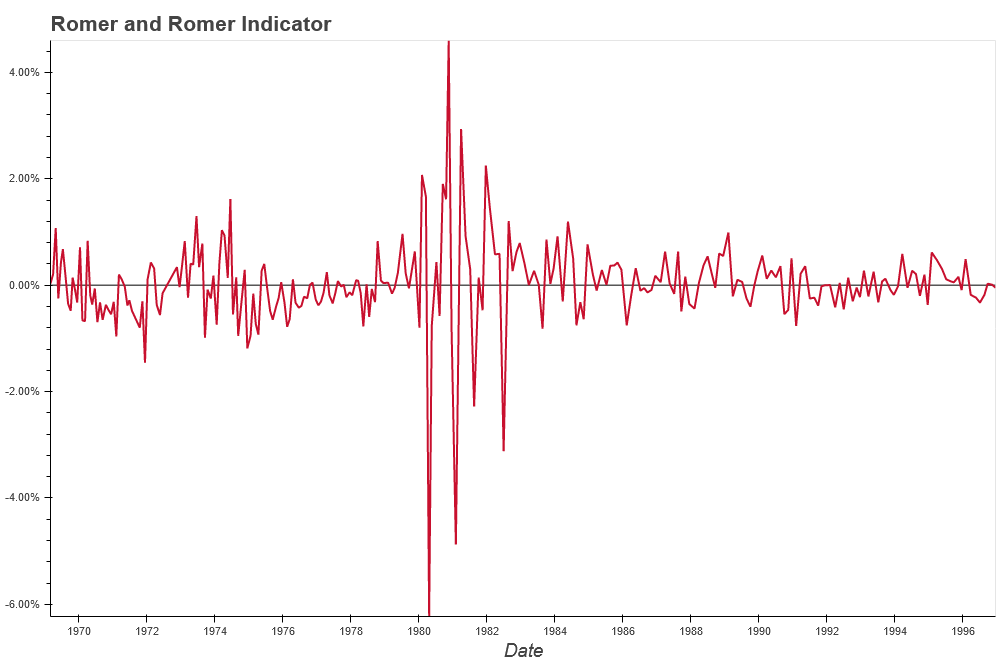
\includegraphics[width=\textwidth]{charts/rr04.png}
		\caption{\label{rr04} The \cite{Romer2004} monetary policy shock time series.}
	\end{figure}
	Note that this model is not intended to be structural and we should not be too interested in the parameter estimates. They are only using the regression to purge endogenous variation in interest rates. RR04 leverage their indicator to estimate an impulse response function describing the effect of a 1\% interest rate hike on a measure of real output and the price level. Essentially, this is an attempt to describe a dynamic income-savings curve in a standard New Keynesian model. 
	
	GK15 uses the more modern high frequency identification strategy described earlier. Information about monetary policy is disproportionately released to the public in tight windows of time. 10 minutes before any FOMC decision is announced, the price of FFR futures should reflect market expectations of interest rates conditional on all the information available to market participants at that time. 20 minutes after the announcement, market participants will update their forecasts conditional on the new information contained in the announcement. Taking the difference between these two prices yields a measure of unexpected changes in interest rates. If the Fed hikes rates, firms will have no reason to change their production plans if they already planned for rate hikes. Standard macroeconomic theory suggests that market actors will only change their behavior in response to unexpected changes in interest rates. Therefore, GK15's methodology allows us to identify exogenous variation in interest rates.
	\begin{figure}
		\centering
		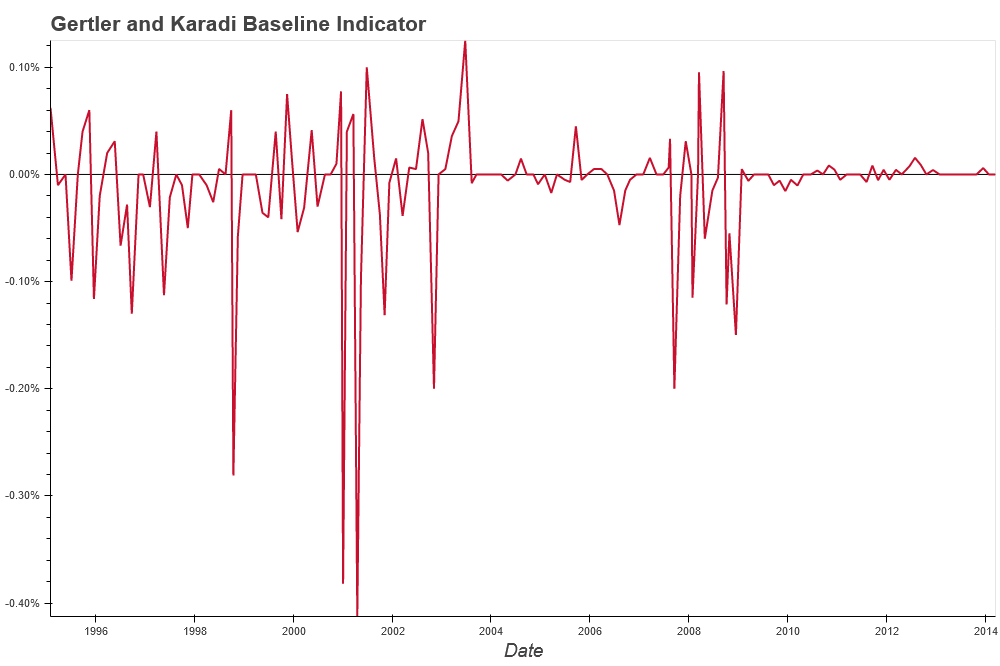
\includegraphics[width=\textwidth]{charts/gk15.png}
		\caption{\label{gk15} The surprise in the 3 month ahead FFR futures rate \citep{Gertler2015}.}
	\end{figure}
	
	Like RR04, GK15 estimates the dynamic IS curve to determine the effect of interest rate hikes on real output over time. RR04 uses two different approaches to do so: a time series model and a vector auto-regression (VAR). GK15 only uses a VAR. As such, the VAR estimates will provide the most consistent comparison between the two indicators. In response to a 1\% increase in interest rates, the RR04 indicator implies a peak impact of -2.9\% real output growth at 23 months while the baseline GK15 indicator implies a peak impact of -2.0\% at 15 months. Consistent with macroeconomic intuition on the long run neutrality of money, the impact of both indicators declines to zero eventually. In principle, these indicators should be measuring the same thing, so a question arises: what explains the difference?  
	
	\cite{Bauer2020} may shed some light. They analyze evidence for and against what they call the Fed-information effect. They argue that indicators based on high frequency financial market "surprises" could be contaminated by omitted variable bias if the FOMC releases information about the state of the economy with each of their announcements. They analyze the effect of the \cite{Nakamura2018} indicator (very similar to GK15) on private sector forecasts of state variables. Bauer and Swanson's position is that there is weak evidence for the Fed information effect and instead provide an alternative theory that the Fed is responding to news at the same time market participants are. Among many other tests, they regress high frequency changes in the price of S\&P500 ETFs on the Nakamura indicator and test for a statistically significant negative slope. If markets react positively to rate hikes, then that is strong evidence for the Fed information effect. With this particular test, they find no evidence for the Fed-information effect. 
	
	I believe there are serious problems with this approach. On theoretical grounds, it assumes some form of irrational expectations. Market participants have to be persistently "tricked" in order for their hypothesis to work. Moreover, I do not believe the S\&P500 test is sufficient to reject the possibility of endogeneity or even the possibility that the Fed information effect is large. Omitted variable bias will cause our parameter estimates to be inconsistent and biased, but we cannot know how large the bias will be just by running the endogenous regression. 
	
	That being said, Bauer and Swanson's approach provides a starting point. The strength of the RR04 indicator is that it purges the Fed's private information about the economy away from changes in interest rates. The Fed-information effect should not be a problem for this indicator. The strength of the GK15 indicator is that it purges private sector information about monetary policy away from changes in interest rates. The GK15 indicator has a more solid theoretical justification based on micro-foundations and rational expectations. Even if the Fed's information about the economy is better than the private sector's, we are interested in understanding the behavior of the private sector. Market actors only make decisions based on the information they have. If the GK15 indicator is contaminated by the Fed-information effect, we can potentially combine the two approaches by replacing the \(\Delta ff_m\) term in equation \ref{eq1} with the GK15 indicator. A new, purified indicator can be derived. With this new indicator, we can repeat the \cite{Bauer2020} regression for both the purified indicator and the baseline GK15 indicator and determine how much the effect of monetary policy changes.
	\section{Economic Theory}
	The Federal Reserve conducts monetary policy primarily through changes in certain benchmark interest rate targets such as the Federal Funds rate. However, rational agents will anticipate the Fed's behavior and make decisions based on their forecasts of the Federal Reserve's future interest rate targets. Therefore, a cut in interest rates may not have any stimulative effect on the economy at all if this rate cut was fully anticipated. The Fed's objective function is based on its forecasts of various state variables in the economy such as unemployment, real output growth, and inflation. Agents will attempt to forecast these same state variables in order to predict the Fed's interest rate target. But markets will only change their behavior they are "surprised" by the Fed's interest rate target. 
	
	As others in the literature have argued \citep{Nakamura2018}, it is very possible that the Fed has information about the economy not available to the public. This creates a potential problem. Even if the Federal Open Market Committee announces an unexpected rate cut, the private sector could be "surprised" just because the FOMC released new information about its forecasts of state variables. For instance, if the FOMC announces an unexpected rate cut but also reveals that it expects unemployment to be much lower than what the private sector expects, the unexpected rate cut may not be expansionary. The rate cut would essentially be explained by the income effect or the Fisher effect, but we want to identify interest rate changes caused by the liquidity effect only. 
	
	In more precise terms, we may model the Fed's nominal interest rate target \(i\) corresponding to an FOMC meeting \(m\) as:
	\begin{align*}
		i_m = i_m^p(\text{PubInfo}_m) + X_m(\text{FedInfo}_m)^\prime \alpha + \epsilon_m \tag{2} \label{struct_mod1}
	\end{align*}
	Where \(i_m^p\) is the private sector's forecast of \(i_m\) given all publicly available information \(\text{PubInfo}_m\) \textit{before} the policy decision is announced, \(X_m\) is a vector of the Fed's forecast of state variables given its private information \(\text{FedInfo}_m\), and \(\epsilon_m\) is an exogenous monetary policy shock. Many in the literature have argued that we may exploit the price of Federal Funds rate futures contracts to estimate \(\epsilon_m\) \citep{Gurkaynak2011,Gertler2015, Nakamura2018}. Adjusting equation \ref{struct_mod1}:
	\begin{align*}
		i_m - i_m^p(\text{PubInfo}_m) = X_m(\text{FedInfo}_m)^\prime \alpha + \epsilon_m \\
		FS_m = X_m(\text{FedInfo}_m)^\prime \alpha + \epsilon_m \tag{3} \label{model}
	\end{align*}
	Where \(FS_m\) is the change in the price of FFR futures contracts over a 30 minute window around the policy announcement corresponding to meeting \(m\). \(FS_m\) is used as an estimate of \(\epsilon_m\), leaving \(X_m\) out as an omitted variable. \cite{Bauer2020} investigate the claim that \(X_m\) is correlated with \(FS_m\). If true, this could imply any attempt to use \(FS_m\) to estimate the effect of monetary policy on some dependent variable of interest \(y_m\) will suffer from omitted variable bias:
	\begin{align*}
		y_m &= \beta_0 + \beta_1 \epsilon_m  + v \\
		y_m &= \beta_0 + \beta_1(FS_m - X_m(\text{FedInfo}_m)^\prime \alpha )  + v \\
		y_m &= \beta_0 + \beta_1FS_m - \beta_1 X_m(\text{FedInfo}_m)^\prime \alpha + v \\
		y_m &= \beta_0 + \beta_1FS_m + u \tag{4} \label{eq3} \\ 
		\mathrm{Cov}(FS_m, u) &\neq 0 
	\end{align*}
	This is source of endogeneity is the Fed-information effect.
	\section{Data}
	We have several sources of time-series data. To measure and test the existence of the Fed information effect, we must first derive a "purified" version of \(FS_m\). We will essentially estimate equation \ref{model} and then use the residual \(\hat{\epsilon}_m\) as our indicator of monetary policy shocks. For \(X_m\), we use data from the Federal Reserve's Greenbook forecasts. These forecasts are made publicly available with a lag of 5 years. The forecasts are made before every scheduled FOMC meeting and they inform policy decisions. The forecasts are made under the assumption of no monetary policy shocks. For \(FS_m\) itself, our sample is limited because the data is proprietary. \cite{Gertler2015} have graciously made their data publicly available. We will use the change in the forecast of interest rates implied by three month ahead FFR futures. Each observation of \(FS_m\) is based on the difference between the futures price 20 minutes after the policy decision of FOMC meeting \(m\) is announced and 10 minutes before the announcement. We use a model very similar to that of \cite{Romer2004}:
	\begin{align*}
		FS_m =  \alpha &+ \sum_{i=0}^{2} \gamma_i \widetilde{\Delta y}_{mi} + \sum^2_{i=0} \lambda_i \left(\widetilde{\Delta y}_{mi}-\widetilde{\Delta y}_{m-1,i}\right) \tag{5} \label{ep_hat_model} \\
		&+\sum^{2}_{i=0} \phi_i \tilde{\pi}_{mi} + \sum^2_{i=0} \theta_i \left(\tilde{ \pi}_{mi}-\tilde{ \pi}_{m-1,i}\right) + \rho \tilde{u}_{m0} + \epsilon_m
	\end{align*}
	For variable definitions see table \ref{gbvars}. Several adjustments are made to the Romer and Romer model. All lagged terms are excluded because this represents information already available to the public, but this information should already be purged from \(FS_m\) by assumption. Market prices reflect all information publicly available. Similarly, we exclude the \(ffrb_m\) term because this is also public information and there is little evidence of mean reversion in \(FS_m\). 
	\begin{table}[ht]
		\centering
		\begin{tabular}{p{0.30\linewidth}  p{0.6\linewidth}}
			\toprule
			Variable & Description \\ 
			\midrule  
			\(m\) & FOMC meeting corresponding to the Greenbook forecast and interest rate shock in question. \\
			\(i\) & Forecast horizon relative to meeting \(m\). Data for the current quarter cannot be observed in real time, so \(i=0\) denotes a nowcast. \\
			\(\widetilde{\Delta y}_{mi}\) &  Real GDP growth forecast.\\
			\(\tilde{\pi}_{mi}\)& Inflation forecast.\\
			\(\tilde{u}_{m0}\) & Unemployment nowcast. \\
			\bottomrule
		\end{tabular}
		\caption{Definition of all variables from the Greenbook forecasts in equation \ref{ep_hat_model}. For each difference term \(x_{mi}-x_{m-1,i}\), we are taking a forecast of \(x\) at the \(i\)th quarter ahead of FOMC meeting \(m\) and looking at how the forecast for \(x\) at quarter \(i\) changed since meeting \(m-1\). In other words, we adjust the forecast horizons for meetings \(m\) and \(m-1\) so that the forecasts refer to the same quarter.}
		\label{gbvars}
	\end{table}
	
	After obtaining our indicator, we will then need to estimate the effect of monetary policy on some dependent variable. Typically, monetary policy shock indicators are used to estimate the dynamic effects on real output or inflation. But \cite{Bauer2020} provide a compelling alternative: the change in the logarithm of S\&P500 stock market price index around each FOMC meeting. Indeed, Bauer and Swanson estimate equation \ref{eq3} directly. Unfortunately, due to data limitations we cannot use high frequency prices for this process. The best we can do is use 24 hour changes in the price of the S\&P500. This is not ideal because the change in prices could be contaminated by non-FOMC news such as a BLS job report released on the same day as an FOMC announcement. The findings in \cite{Gurkaynak2011} indicate that for changes in the price of a wide variety of assets, the difference between a 30 window and a 24 hour window is small overall. Furthermore, this would really only cause problems for our purposes if the confounders are correlated with our regressors. 24 hour data on S\&P500 prices is available from \textit{Yahoo Finance}. 
	\section{Empirical Analysis}
	\begin{table}
		\centering
		\begin{tabular}{lrrr}
			\toprule
			{} &  \(FS_m\) &  \(\hat{\epsilon}_m\) & \(\Delta \log{(\text{S\&P500}_m)}\) \\
			\midrule
			count & 110 &          110&       110 \\
			mean  &  -0.0025 &            0.0000 &         0.2031 \\
			std   &   0.0419 &            0.0373 &         1.1636 \\
			min   &  -0.2000 &           -0.1764 &        -3.1111 \\
			25\%   &  -0.0055 &           -0.0115 &        -0.4039 \\
			50\%   &   0.0000 &            0.0008 &         0.0824 \\
			75\%   &   0.0050 &            0.0150 &         0.7170 \\
			max   &   0.1250 &            0.1152 &         4.5630 \\
			\bottomrule
		\end{tabular}
		\caption{Summary statistics for our final dataset. Note that all variables are reported as percentages.}
		\label{SumStats}
	\end{table}
	Summary statistics for all the data used in these regressions are presented in table \ref{SumStats}. There are multiple tests we will run to evaluate the Fed-information effect hypothesis. As mentioned previously, \cite{Bauer2020} estimate the following equation, which will act as our restricted model:
	\[
	\Delta \log{(\text{S\&P500}_m)} = \beta^R_0 + \beta^R_1 FS_m + u \tag{6} \label{rest}
	\]
	Bauer and Swanson argue that a statistically significant slope implies that the Fed information effect does not exist, however I disagree with this interpretation. What we actually need to know is how much the slope coefficient changes when we include the potentially omitted variable: \(\hat{i}_m\) which is imputed from the regression of equation \ref{ep_hat_model}. I will conduct a Wu-Hausman Test based on equation \ref{rest} and also the following equation:
	\begin{align*}
		\Delta \log{(\text{S\&P500}_m)} &= \delta_0 + \delta_1 \hat{\epsilon}_m + w \tag{8} \label{trumod}
	\end{align*}
	Here, equation \ref{trumod} is the most direct representation of the "true model" if the Fed information effect is statistically significant. Note that the exclusion of \(\hat{i}_m\) from equation \ref{trumod} should not make a difference because \(\mathrm{Cov}(\hat{i}_m, \hat{\epsilon}_m) = 0\) by construction.
	\begin{table}[!htbp] \centering
		\begin{tabular}{@{\extracolsep{5pt}}lcc}
			\\[-1.8ex]\hline
			\hline \\[-1.8ex]
			& \multicolumn{2}{c}{\textit{Dependent variable:} \(\Delta \log{(\text{S\&P500}_m)}\)} \
			\cr \cline{2-3}
			\\[-1.8ex] & (1) & (2) \\
			\hline \\[-1.8ex]
			Intercept & 0.002$^{*}$ & 0.002$^{*}$ \\
			& (0.001) & (0.001) \\
			\(FS_m\) & -6.518$^{**}$ & \\
			& (2.601) & \\
			\(\hat{\epsilon}_m\) & & -7.154$^{**}$ \\
			& & (2.919) \\
			\hline \\[-1.8ex]
			Observations & 110 & 110 \\
			$R^2$ & 0.055 & 0.053 \\
			Adjusted $R^2$ & 0.046 & 0.044 \\
			Residual Std. Error & 0.011(df = 108) & 0.011(df = 108)  \\
			F Statistic & 6.280$^{**}$ (df = 1.0; 108.0) & 6.007$^{**}$ (df = 1.0; 108.0) \\
			\hline
			\hline \\[-1.8ex]
			\textit{Note:} & \multicolumn{2}{r}{$^{*}$p$<$0.1; $^{**}$p$<$0.05; $^{***}$p$<$0.01} \\
		\end{tabular}
	\caption{Regression results.}
	\label{finalReg}
	\end{table}

	Regression results are reported in table \ref{finalReg}. The coefficients are fairly close to each other, but there is a surprisingly large difference in standard errors. With these parameter estimates, we can derive the Wu-Hausman test statistic.
	\begin{align*}
		H_0: &\delta_1 \text{ and } \beta_1^R \text{ are consistent.} \\
		H_a: &\delta_1 \text{ is consistent but } \beta_1^R \text{ is inconsistent.} \\
		\text{Test statistic: } &H = \frac{(\hat{\delta}_1-\hat{\beta}_1^R)^2}{\mathrm{Var}(\hat{\delta}_1)-\mathrm{Var}(\hat{\beta}_1^R)} \sim \chi^2_1 \\
		&H = \frac{( -7.154+6.518)^2}{2.919^2- 2.601^2} = .2304
	\end{align*}
	Our Wu-Hausman test statistic implies a P-value of 63.12\%, which is statistically insignificant. We have insufficient evidence to reject our null hypothesis.
	\section{Conclusion} 
		Understanding the strength of monetary policy is crucially important for the purpose of macroeconomic stabilization. Endogeneity is always a concern when constructing monetary policy indicators. The Fed-information effect would imply our estimates of the effectiveness of monetary policy is systematically biased and attenuated. The literature is divided on whether this effect actually exists. \cite{Nakamura2018} argue that the Fed information effects exists and while \cite{Bauer2020} come to the opposite conclusion. Based on the above results, I find no evidence that the Fed-information effect exists.
		
		I find these results rather surprising. The premise of the Fed-information effect is highly sound on theoretical grounds and very plausible based on the relative accuracy of the Federal Reserves forecasts over private sector forecasts as found in \cite{Romer2000}. One possible explanation is that the sample of Romer and Romer's 2000 paper is too narrow. Their largest samples cover less than 10 years of data from the 1990s, whereas my sample covers 14 years of more recent data. Its possible Romer and Romer's paper has an external validity problem - neither the private sector nor the Fed's forecasts are static. They both improve forecasts over time based on the accuracy of previous forecasts. Its possible that the gap in accuracy has closed over time, meaning the Fed has less private information hidden from the public. This in and of itself may have implications for monetary policy makers.
		
		The central argument of \cite{Nakamura2018} is based on how forecasts from the \textit{Blue Chip Economic Indicators} survey change in response to monetary policy surprises. For example, they find that inflation forecasts tend to increase after unexpected rate hikes, inconsistent with macroeconomic intuition. The discrepancy with my results could be explained by the fact that our data uses a much tighter window. This is crucial for our identification strategy. By limiting our window of stock price changes to only 24 hour changes, we can be more confident that we exclude any confounding factors. But the \textit{Bluechip} forecasts are monthly forecasts, so we do not have a good idea of what it is that the forecasters are responding to. 
		
		Another explanation is provided by \cite{Bauer2020} who agree with our results. They argue the \textit{Bluechip} forecasters are responding to the same news that the Fed is responding to when the Fed makes decisions. Despite our concurring results, I think this alternative explanation is still highly implausible. Market participants are highly responsive to all economic news \citep{Gurkaynak2011}, but the Bauer and Swanson model assumes that market participants delay trading until the day of an FOMC announcement, leaving a large arbitrage opportunity for quite a long time. My reservations aside, my results provide some indirect evidence for their model. If their model is correct then there may be much larger policy implications. In \cite{Bauer2020}, they estimate the dynamic IS curve using their "Fed-response to news" model and find that the impact of monetary policy peaks in less than one year.
		
		Further research is warranted. The biggest weakness of our paper is our window for stock market price changes. High frequency data is available but not free. The robustness of our results will increase substantially if we use the same 30 minute from the FFR futures changes for stock market price changes. In addition, I believe its necessary to do more research on the relative "quality" of the Fed's information. Extending the sample of \cite{Romer2000} will go a long way in this regard. In addition, its possible that stock market prices may not be the best dependent variable. High frequency TIPs spread data could give us an idea of how market forecasts of inflation change directly. 
		
		The main contribution of this research is a method of not only testing the Fed-information effect but also measuring how important the Fed-information effect actually is. The null result challenges a portion of the existing literature and alternative explanation offer a wide frontier of opportunities for new research.
		\bibliography{refs}
\end{document}